\documentclass{report}

\usepackage[utf8]{inputenc} % Charakter-Kodierung
\usepackage[german]{babel} % Sprache

\usepackage[table,xcdraw]{xcolor} % Tabellen Farben
\usepackage{tabularx} % Dynamische Tabellenbreite
\usepackage{tcolorbox} % Graue Boxen
\usepackage{hyperref} % url Umgebung
\usepackage{todonotes} % Notizen
\usepackage{natbib} % Bibliographie
\usepackage{fancyhdr} % Header und Footer
\usepackage{multirow} % Multizeile
\usepackage{geometry} % Page layout
\usepackage{color} % Text Farben

% Page layout
\geometry{
	bottom=3.5cm,
	headheight=180pt
}

% Nummerierung der ersten Seiten verhindern
\pagenumbering{gobble}

% Bibstyle
\bibliographystyle{plain}

% Header / Footer
\fancypagestyle{plain}{
	\fancyhf{}% Clear header/footer
	\fancyhead[R]{
\includegraphics[width=4cm]{img/cau-logo-2017}} % Rechter header
	\fancyhead[L]{\leftmark} % Linker header
	\fancyfoot[R]{\thepage} % Rechter footer
	\fancyfoot[L]{
\includegraphics[width=1cm]{img/se-logo}} % Linker footer	
}
\pagestyle{plain}

\renewcommand{\headrulewidth}{0.5pt} % Unnötige Informationen der Kapitelangabe
\renewcommand{\footrulewidth}{0.2pt} % entfernen
\renewcommand{\chaptermark}[1]{\markboth{{#1}}{}}




% Zahlen für Fußnoten
\renewcommand{\thefootnote}{\arabic{footnote}}
\renewcommand{\thempfootnote}{\arabic{mpfootnote}}

%%%%% Ausfüllen %%%%%

% Gruppenname
\newcommand{\gruppenname}{Gruppe X}

% Projektname
\newcommand{\projektname}{Projektname}

% Semester
\newcommand{\semester}{SoSe17}



% Titelseite

\title{
	\vspace*{-3cm}
	Pflichtenheft\\
	\projektname\\
	-\\
	\color{gray}
	Softwareprojekt \semester\\
	\gruppenname\\
	\vspace*{5mm}
	
\includegraphics[width=\textwidth]{img/logo}
}

\author{
	\begin{tabular}{r l@{\hspace{8\tabcolsep}} r} 
		Vorname1 & Nachname1 & \multirow{8}{*}{ 
\includegraphics{img/se-logo} } \\
		Vorname2 & Nachname2 \\
		Vorname3 & Nachname3 \\
		Vorname4 & Nachname4 \\
		Vorname5 & Nachname5 \\
		Vorname6 & Nachname6 \\
		Vorname7 & Nachname7 \\
		Vorname8 & Nachname8 \\
	\end{tabular}
}

\date{\today}





% Dokument

\begin{document}
	\maketitle
	
	%%%% Bitte löschen oder auskommentieren %%%%
	%%%%%%%%% Dient nur als Hilfe %%%%%%%%%%
	
	\chapter*{Tipps und Hilfen}\label{chp:tipps}
	\vspace*{-1cm}
	\begin{tcolorbox}
		\textbf{Information:} Dieses Kapitel und alle folgenden grauen Boxen dienen als Hilfestellungen und sollen im fertigen Dokument nicht enthalten sein. 
		%
		\\\\
		%
		Zur Versionsverwaltung während des Softwareprojekts muss \textit{Git} genutzt werden.
		Git führt Textdokumente mit unterschiedlichen Zeilenbearbeitungen automatisch zusammen.
		Wir empfehlen den Einsatz von \LaTeX~für alle Textdokumente.
		Um das Auto-Merging zu unterstützen, sollte nach jedem Satzende eine neue Zeile im Quelltext begonnen werden.
		Die .tex-Datei dieser PDF verdeutlicht dies.
		Erkennt Git, dass eine gleiche Zeile bearbeitet wurde, wird ein Konflikt auftreten.
		Dieser kann in der entsprechenden Datei von Hand mittels eines Texteditors behoben werden.
		%
		\\\\
		%
		Fußnoten\footnote{\url{https://www.se.informatik.uni-kiel.de/en}} werden für Homepages genutzt.
		Zitierungen können mittels eines \textit{cite}-Befehls gesetzt, z.B. \textit{citep}~\citep{Shaw2003WritingGoodSoftwareEngineeringesearchPapersMinitutorial}.
		%
		\\\\
		%
		Tipps zur UML-Modellierung können im SE-Wiki\footnote{\url{https://git.informatik.uni-kiel.de/ag-se/teaching-public/wikis/home}} nachgelesen werden.
		Achtet darauf, dass eure Diagramme stets lesbar (Vektor-Grafiken!) und gut strukturiert sind.
		Oftmals ist es sinnvoll ein bis zwei Sätze zusätzlich für Diagrammelemente zu formulieren.
		So können Missverständnisse ausgeschlossen werden, was einen Einfluss auf die Korrektur haben kann.
		Diagramme für unwichtige Tätigkeiten (z.B. Login / Logout, User erstellen / löschen, Passwort ändern etc.) sind nicht erforderlich.	
	\end{tcolorbox}
	
	\todo[inline]{So kann eine TODO-Notiz erzeugt werden}
	
	\begin{figure}[h]
		\centering
		\missingfigure{So kann eine Placeholder-Grafik beispielsweise in den Text eingefügt werden.}		
		\caption{Beschreibung}
		\label{fig:x}
	\end{figure}
		
	%%%%%%%%%%%%%%%%%%%%%%%%%%%%%%
	
	\tableofcontents
	
	\chapter{Lizenz}\label{chp:lizenz}
	\pagenumbering{arabic} % Nummerierung starten
	Copyright 2018 Jette Petzold, Jeremia B\"{o}hmig, Connor Sch\"{o}nberner, Robert K\"{o}hler, Christian Richter, Janek Haberer, Felix Gr\"{o}ner, Johanna Menzel\\
\\Lizenziert unter Apache License, der Version 2.0 (im Folgenden Lizenz); es ist nicht gestattet die Software au\ss{}erhalb der durch die Lizenz festgelegten Bestimmungen zu verwenden.
Die volle Lizenz ist einsehbar unter
\begin{quote}
	http://www.apache.org/licenses/LICENSE-2.0
\end{quote}
Sofern nicht anders durch geltendes Gesetz vorgeschrieben oder schriftlich vereinbart, erfolgt die Verteilung der Software unter dieser Lizenz so wie sie hier vorzufinden ist, ohne jedwede explizite oder implizite Garantien oder Bedingungen.
Zur Kenntnisnahme des genauen Wortlauts der Lizenz ist die Lizenz unter dem angegebenen Link einzusehen.


	
	\chapter{Zielbestimmungen}\label{chp:zielbestimmungen}
	Im Folgenden ist der Funktionsumfang des SWARM Composers, insbesondere der Web-App und der Android-App, aufgeführt. Dabei werden funktionale und nicht-funktionale Zielbestimmungen getrennt aufgeführt. Des Weiteren wird zwischen Muss-, Soll-, Kann- und Abgrenzungskriterien unterschieden.
%
\begin{itemize}[leftmargin=4pc]
	\item Musskriterien umfassen alle Ziele und Funktionalitäten, die für einen Einsatz des entwickelten Produktes unabdingbar sind.
	Sie müssen daher ohne Kompromisse implementiert werden. Ein Wegfall eines einzelnen Musskriteriums würde das Produkt außer Betrieb setzen.
	\item Sollkriterien sind gewünschte Funktionen, die ebenfalls implementiert werden müssen, deren Wegfall auf Grund von unüblichen Umständen aber nicht den Einsatz des Produkts hindern würde.
	\item Kannkriterien sind alle Ziele, die wünschenswert sind, aber nicht zwingend notwendige Funktionen darstellen. 
	\item Abgrenzungskriterien zeigen, was explizit \textbf{nicht} umgesetzt wird. Sie dienen dazu die Grenzen des Produkts zu definieren.
	\\\\
\end{itemize}
%

\textbf{Funktionale Zielbestimmungen}\newline
%

\textit{Musskriterium}

\begin{itemize}[leftmargin=4pc]
	\item Der SWARM Composer muss über eine native Android-App erreichbar sein.
	\item Der SWARM Composer muss über eine Website erreichbar sein.
	\item Auf der Website muss die Möglichkeit bestehen, Kompositionen zu erstellen.
	\item Es muss die Möglichkeit geben, über eine REST-Schnittstelle Dienste einzulesen.
	\item Der SWARM Composer muss eine Kompatibilitätsprüfung für Kompositionen durchführen.
	\item Es muss eine grafische Rückmeldung über die Kompatibilität von Diensten geben.
	\item Die Speicherung von erstellten Kompositionen muss möglich sein.
	\item Die Android-App muss erstellte Kompositionen anzeigen können.
	\item Neue Benutzer des SWARM Composers müssen über die Website registriert werden können.
	\item Registrierte Benutzer des SWARM Composers müssen sich anmelden können, unabhängig davon, ob sie über die Website oder die Android-App zugreifen.
	\item Beim manuellen Erstellen von Diensten muss das Format überprüft werden.
\end{itemize}

\textit{Sollkriterium}

\begin{itemize}[leftmargin=4pc]
	\item Unter allen Nutzern soll zwischen zwei Rollen, normaler Nutzer und Administrator, unterschieden werden, wobei letzterer mehr Nutzungsrechte hat.
	\item Die Website soll für Administratoren die Möglichkeit bieten, Dienste manuell dem System hinzuzufügen.
	\item Der Ersteller einer Komposition soll festlegen können, welche anderen Benutzer diese sehen können.
	\item Der Ersteller einer Komposition soll festlegen können, welche anderen Benutzer diese verändern können.
	\item In der Android-App soll die Möglichkeit bestehen, Kompositionen zu verschicken.
\end{itemize}

\textit{Kannkriterium}

\begin{itemize}[leftmargin=4pc]
	\item Die Android-App kann einzelne Dienste anzeigen.
	\item Es können Alternativen angezeigt werden, wenn Dienste nicht kompatibel sind.
	\item Es gibt eine Suchfunktion für Dienste und Kompositionen.
	\item Auf der Website können Konfigurationen verschickt werden.
\end{itemize}

\textit{Abgrenzungskriterium}

\begin{itemize}[leftmargin=4pc]
	\item In der Android-App können keine Kompositionen erstellt werden.
	\item In der Android-App können keine Dienste erstellt werden.
	\item In der Android-App können keine Benutzer registriert werden.
	\item Beim manuellen Erstellen von Diensten wird nicht geprüft, ob der Inhalt korrekt ist.
	\item Es gibt keine benutzerspezifische Auswahl von Diensten.\\
\end{itemize}


\textbf{nicht funktionale Zielbestimmungen}\newline

\textit{Musskriterium}

\begin{itemize}[leftmargin=4pc]
	\item Die Web-Applikation muss mit Java-Spring erstellt werden.
	\item Die Android-App muss ab der Android Version 6 benutzbar sein.
	\item Die verwendeten URLs müssen zur Laufzeit änderbar sein.
\end{itemize}

\textit{Sollkriterium}

\begin{itemize}[leftmargin=4pc]
	\item Die Kommunikation zwischen Web-App und Android-App soll veschlüsselt sein.
	\item Es soll eine Drag and Drop Benutzeroberfläche auf der Website geben.
	\item Die Benutzeroberfläche soll einfach und intuitiv gestaltet sein.
	\item Der Quellcode des SWARM Composers soll unter eine geeignete Lizenz gestellt werden.
\end{itemize}


	
	\chapter{Produkteinsatz}\label{chp:produkteinsatz}
	\section*{Anwendungsgebiete}
Der SWARM Composer dient Anwender*Innen des BIMSWARM-Ökosystems dazu, Kompositionen von Diensten auf ihre Kompatibilität zu prüfen. Über das Ergebnis dieser Prüfung gibt das System grafisch eine Rückmeldung. Gleichzeitig lässt sich mit ihm ein Überblick über die vorhandenen atomaren Dienste erlangen sowie Kompositionen verwalten. 

\section*{Zielgruppen}

Primär richtet sich der SWARM Composer an Benutzer*Innen aus der Architektur- und Baubranche, ohne dass weiteres Zusatzwissen über die interne Funktionsweise des Systems vorausgesetzt ist. Allerdings ist Wissen über übliche Services, die im SWARM-Ökosystem genutzt werden, hiflreich, um Kombinationen zu erstellen.

Es sind zwei Rollen vorgesehen: Zum einen Standard-User, die sowohl Dienste zu Kompositionen zusammensetzen als auch diese prüfen, speichern und teilen, zum anderen Admin-User, die zusätzlich Dienste anlegen können. Ein Admin muss hierfür das von Adesso spezifizierte Format für Dienste kennen.

\section*{Betriebsumgebungen}

Zum Betrieb des Systems ist ein Server-Computer, auf dem die Webanwendung laufen kann, zwingend notwendig. Wenn die Nutzung der App gewünscht ist, ist hierfür ein Android-Mobilgerät in Form eines Tablets oder Smartphones notwendig. Für die auf einem Server (beispielsweise in Form von Apache Tomcat) laufende Anwendung ist ganztägige Uptime und autonomes Laufen gewährleistet. Es findet automatische Datensicherung statt.





		
	\chapter{Produktumgebung}\label{chp:produktumgebung}
	Um die Software fehlerfrei und korrekt zu nutzen, müssen bestimmte technische Bedingungen erfüllt sein, die hier aufgeführt werden.

\section{Software}

Für das Webinterface dient ein einfacher Webbrowser als Client.
Um die App zu benutzen, wird Android 6.0 oder neuer vorausgesetzt.
\newline
\newline
Auf dem Server muss eine Linux-Distribution mit Docker und Jenkins installiert sein.

\section{Hardware}

Für die App muss das Gerät Android 6.0 oder neuer unterstützen.
\newline
\newline
Webservices müssen auf dem Server laufen können.


\section{Orgware}

Sowohl Server als auch die Clients müssen netzwerkfähig sein.


\section{Produktschnittstelle}

Die Kommunikation zwischen Server und Client findet bei dem Webinterface über HTTPS und bei der App über eine REST-Schnittstelle statt. Für das Verschicken von exportierten Pdfs wird die Standard Android API verwendet.
	

	\chapter{Produktfunktionen}\label{chp:produktfunktionen}
	Die Produktfunktionen beschreiben jede einzelne Funktion des Produkts mittels Anwendungsfalldiagrammen und Anwendungsfalltabellen.
\\\\
In  Tabelle~\autoref{fig:akteur-tabelle} werden alle auftretenden Akteure beschrieben.


\begin{figure}[h]
	\centering

	\begin{tabularx}{\textwidth}{ p{.2\textwidth} | p{.4\textwidth} | X }
		\textbf{Akteur} & \textbf{Beschreibung} & \textbf{Verwendet in Anwendungsszenario} \\ \hline
		unregistriertr Nutzer & Nicht angemeldete Nutzer: Kann nur Kompositionen einsehen & APP-2, APP-3, WEB-6
		\\ \hline Nutzer & Angemeldeter Nutzer: Nutzt den SWARM Composer & APP-1, APP-2, APP-3, APP-4, WEB-4, WEB-5, WEB-6
		\\ \hline Administrator & Nutzt und verwaltet den SWARM-Composer & APP-1, APP-2, APP-3, APP-4, WEB-1, WEB-2, WEB-3, WEB-4, WEB-5, WEB-6
	\end{tabularx}

	\caption{Beschreibung der Akteure}
	\label{fig:akteur-tabelle}
\end{figure}


%%%%%%%%%%%%%%%
%% Anwendungsfall 1 %%
%%%%%%%%%%%%%%%
\newpage

\section{Anwendungsfalldiagramm - App}

\begin{figure}[h]
	\centering	
	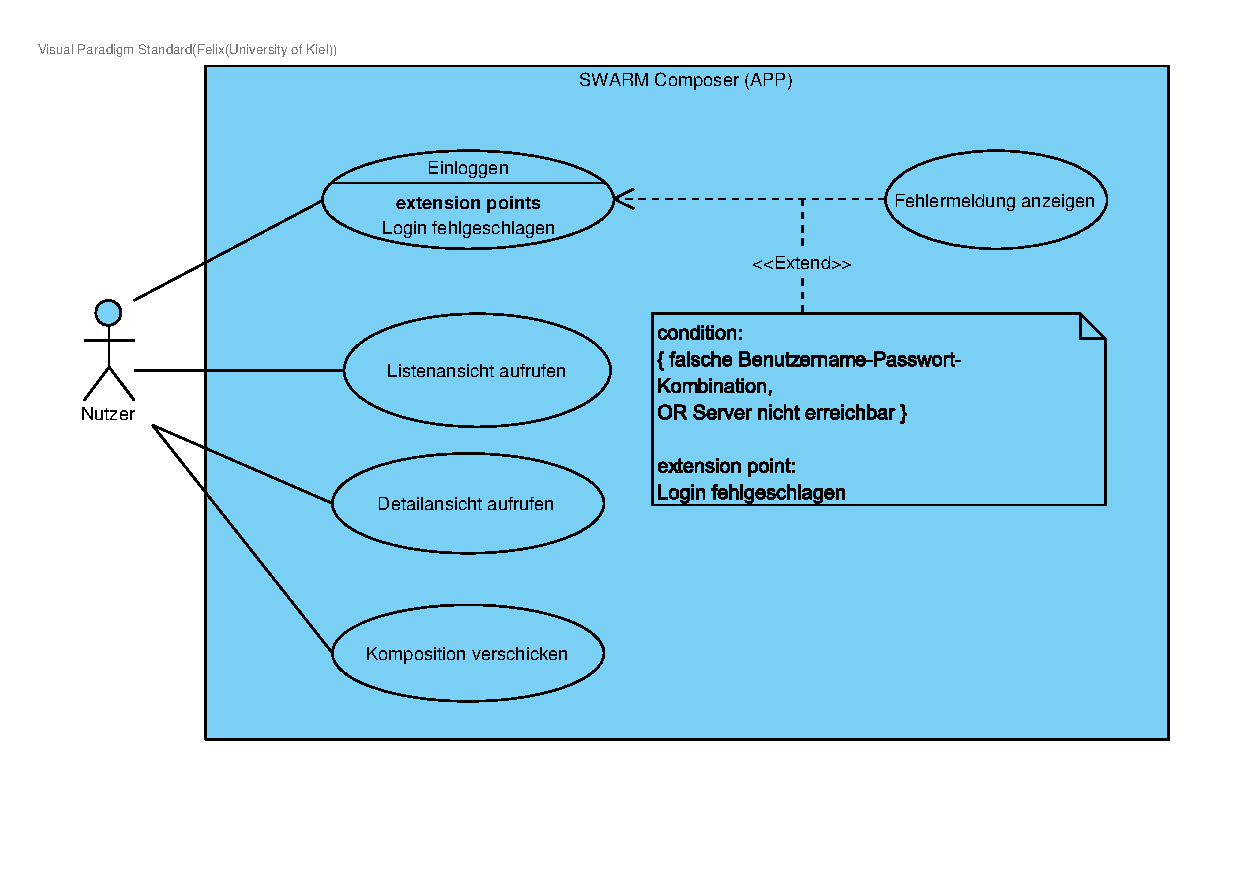
\includegraphics[width=\textwidth]{img/Produktfunktionen_app}	
	\caption{Anwendungsfalldiagramm - App}
	\label{fig:anwendungsfalldiagramm-app}
\end{figure}

\newpage

\begin{figure}[h]
	\centering
	\begin{tabularx}{\textwidth}{ X | X }
		\textbf{Anwendungsfall ID} & APP-1 \\ \hline
		\textbf{Anwendungsfallname} & Einloggen \\ \hline
		\textbf{Initiierender Akteur} & Ein Nutzer \\ \hline
		\textbf{Weitere Akteure} & -  \\ \hline
		\textbf{Kurzbeschreibung} & Ein Nutzer loggt sich ein. \\ \hline
		\textbf{Vorbedingungen} & Android-App ist geöffnet, der Nutzer ist nicht eingeloggt. \\ \hline
		\textbf{Nachbedingungen} & Der Nutzer ist eingeloggt. \\ \hline
		\textbf{Ablauf} &
			\begin{enumerate}
				\item Der Nutzer gibt seinen Benutzernamen ein
				\item Der Nutzer gibt sein Passwort ein
				\item Der Nutzer tippt auf den Login-Button
				\item Bestätigung der erfolgreichen Anmeldung wird angezeigt.
			\end{enumerate} \\ \hline
		\textbf{Alternative} &
				- \\ \hline
		\textbf{Ausnahme} &
				\begin{enumerate}
					\item Der Nutzer gibt den Benutzernamen ein.
					\item Der Nutzer gibt das Passwort ein.
					\item Der Nutzer tippt auf den Login-Button.
					\item Anmeldung schlägt fehl und eine Fehlermeldung wird angezeigt.
				\end{enumerate}  \\ \hline
		\textbf{Benutzte Anwendungsfälle} & Fehlermeldung anzeigen \\ \hline
		\textbf{Spezielle Anforderungen} & - \\ \hline
		\textbf{Annahmen} & -
	\end{tabularx}
	\caption{Anwendungsfall APP-1}
	\label{fig:anwendungsfall-app-tabelle-APP-1}
\end{figure}

\newpage

\begin{figure}[h]
	\centering
	\begin{tabularx}{\textwidth}{ X | X }
		\textbf{Anwendungsfall ID} & APP-2 \\ \hline
		\textbf{Anwendungsfallname} & Listenansicht aufrufen \\ \hline
		\textbf{Initiierender Akteur} & Nutzer \\ \hline
		\textbf{Weitere Akteure} & -  \\ \hline
		\textbf{Kurzbeschreibung} & Dem Nutzer wird eine Liste von vorhandenen Kompositionen angezeigt \\ \hline
		\textbf{Vorbedingungen} & Android-App ist geöffnet  \\ \hline
		\textbf{Nachbedingungen} & Dem Nutzer wird eine Liste von vorhandenen Kompositionen angezeigt  \\ \hline
		\textbf{Ablauf} &
		\begin{enumerate}
			\item Die für den Nutzer sichtbaren Kompositionen werden vom Server abgerufen
			\item Daten werden als Liste angezeigt.
		\end{enumerate} \\ \hline
		\textbf{Alternative} &
		\begin{enumerate}
			\item Der Nutzer kehrt zur Listenansicht zurück.
			\item Dem Nutzer wird eine Liste der sichtbaren Kompositionen angezeigt.
		\end{enumerate}  \\ \hline
		\textbf{Ausnahme} &
		-  \\ \hline
		\textbf{Benutzte Anwendungsfälle} & - \\ \hline
		\textbf{Spezielle Anforderungen} & - \\ \hline
		\textbf{Annahmen} & -
	\end{tabularx}
	\caption{Anwendungsfall APP-2}
	\label{fig:anwendungsfall-app-tabelle-APP-2}
\end{figure}

\newpage

\begin{figure}[h]
	\centering
	\begin{tabularx}{\textwidth}{ X | X }
		\textbf{Anwendungsfall ID} & APP-3 \\ \hline
		\textbf{Anwendungsfallname} & Detailansicht aufrufen \\ \hline
		\textbf{Initiierender Akteur} & Nutzer \\ \hline
		\textbf{Weitere Akteure} & -  \\ \hline
		\textbf{Kurzbeschreibung} & Nutzer ruft die Detailansicht einer Komposition auf  \\ \hline
		\textbf{Vorbedingungen} & Nutzer hat die Listenansicht aufgerufen.  \\ \hline
		\textbf{Nachbedingungen} & Nutzer wird die Detailansicht einer Komposition gezeigt \\ \hline
		\textbf{Ablauf} &
		\begin{enumerate}
			\item Nutzer wählt in der Listenansicht eine Komposition aus.
			\item Nutzer werden die Details der ausgewählten Komposition angezeigt.
		\end{enumerate} \\ \hline
		\textbf{Alternative} &
		-  \\ \hline
		\textbf{Ausnahme} &
		- \\ \hline
		\textbf{Benutzte Anwendungsfälle} & - \\ \hline
		\textbf{Spezielle Anforderungen} & - \\ \hline
		\textbf{Annahmen} & -
	\end{tabularx}
	\caption{Anwendungsfall APP-3}
	\label{fig:anwendungsfall-app-tabelle-APP-3}
\end{figure}

\newpage

\begin{figure}[h]
	\centering
	\begin{tabularx}{\textwidth}{ X | X }
		\textbf{Anwendungsfall ID} & APP-4 \\ \hline
		\textbf{Anwendungsfallname} & Komposition verschicken \\ \hline
		\textbf{Initiierender Akteur} & Nutzer
		 \\ \hline
		\textbf{Weitere Akteure} & -  \\ \hline
		\textbf{Kurzbeschreibung} & Nutzer verschickt eine Komposition.  \\ \hline
		\textbf{Vorbedingungen} & Nutzer hat in der Listenansicht eine Komposition ausgewählt und die Detailansicht aufgerufen.  \\ \hline
		\textbf{Nachbedingungen} & Komposition wird verschickt  \\ \hline
		\textbf{Ablauf} &
		\begin{enumerate}
			\item Nutzer wird eine Komposition in der Detailansicht angezeigt.
			\item Nutzer tippt auf den Verschicken-Button.
			\item Eine Datei im PDF-Format wird erstellt.
			\item Nutzer bestätigt den Versand.
		\end{enumerate} \\ \hline
		\textbf{Alternative} &
		-  \\ \hline
		\textbf{Ausnahme} &
		- \\ \hline
		\textbf{Benutzte Anwendungsfälle} & - \\ \hline
		\textbf{Spezielle Anforderungen} & - \\ \hline
		\textbf{Annahmen} & -
	\end{tabularx}
	\caption{Anwendungsfall APP-4}
	\label{fig:anwendungsfall-app-tabelle-APP-4}
\end{figure}

\newpage

%%%%%%%%%%%%%%%
%% Anwendungsfall 2 %%
%%%%%%%%%%%%%%%

\section{Anwendungsfalldiagramm - Server}

\begin{figure}[h]
	\centering
	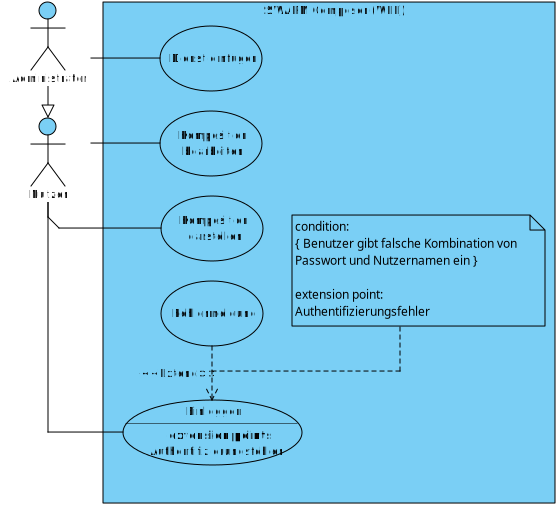
\includegraphics[width=\textwidth]{img/Produktfunktionen_web}
	\caption{Anwendungsfalldiagramm - Server}
	\label{fig:anwendungsfalldiagramm-server}
\end{figure}

\newpage

\begin{figure}[h]
	\centering
	\begin{tabularx}{\textwidth}{ X | X }
		\textbf{Anwendungsfall ID} & WEB-1 \\ \hline
		\textbf{Anwendungsfallname} & Dienst manuell einfügen \\ \hline
		\textbf{Initiierender Akteur} & Administrator \\ \hline
		\textbf{Weitere Akteure} & - \\ \hline
		\textbf{Kurzbeschreibung} & Neuer Dienst wird in die Datenbank eingefügt \\ \hline
		\textbf{Vorbedingungen} & Administrator ist eingeloggt und befindet sich auf Administrationsseite \\ \hline
		\textbf{Nachbedingungen} & Neuer Dienst wurde in Datenbank gespeichert \\ \hline
		\textbf{Ablauf} &
		\begin{enumerate}
			\item [1.] [Use-Case: Authentifizieren]
			\item [2.] Administrator wählt ``Dienst eingeben'' aus
			\item [3.] Administrator gibt Dienstdetails in Eingabemaske ein
			\item [4.] Administrator bestätigt die Eingabe.
			\item [5.] System akzeptiert Eingabe und speichert in Datenbank.
			\item [6.] Weiterleitung zur Administrationsseite
		\end{enumerate} \\ \hline
		\textbf{Alternative} & - \\ \hline
		\textbf{Ausnahme} &
		\begin{enumerate}
			\item [1.] [Use-Case: Authentifizieren]
			\item [2.] Administrator wählt ``Dienst eingeben'' aus
			\item [3.] Administrator gibt Dienstdetails in Eingabemaske ein
			\item [4.] Administrator bestätigt die Eingabe.
			\item [5.] System akzeptiert Eingabe nicht, da sie syntaktisch ungültig ist.
			\item [6.] System zeigt Fehler an und markiert ungültig Felder.
			\item [7.] Es wird in der Eingabemaske verblieben.
		\end{enumerate} \\ \hline
		\textbf{Benutzte Anwendungsfälle} & Authentifizieren \\ \hline
		\textbf{Spezielle Anforderungen} & - \\ \hline
		\textbf{Annahmen} & Authentifizierung ist erfolgreich
	\end{tabularx}
	\caption{Anwendungsfall WEB-1}
	\label{fig:anwendungsfall-server-tabelle-web-1}
\end{figure}

\begin{figure}[h]
	\centering
	\begin{tabularx}{\textwidth}{ X | X }
		\textbf{Anwendungsfall ID} & WEB-2 \\ \hline
		\textbf{Anwendungsfallname} & Dienste einlesen \\ \hline
		\textbf{Initiierender Akteur} & Administrator \\ \hline
		\textbf{Weitere Akteure} & - \\ \hline
		\textbf{Kurzbeschreibung} & Ein oder mehrere Dienste werden über eine JSON Datei eingelesen, die sich lokal auf einem Nutzerrechner befindet \\ \hline
		\textbf{Vorbedingungen} & Administrator ist eingeloggt und befindet sich auf der Administrationsseite \\ \hline
		\textbf{Nachbedingungen} & Neue Dienste wurden der Datenbank hinzugefügt \\ \hline
		\textbf{Ablauf} &
		\begin{enumerate}
			\item [1.] [Use-Case: Authentifizieren]
			\item [2.] Administrator wählt ``Dienste einlesen'' aus
			\item [3.] Administrator wählt die hochzuladene JSON-Datei aus dem sich öffnenden Dateibrowser vom lokalen Rechner aus
			\item [4.] Eingelesene Daten werden vom System akzeptiert und aufgelistet
			\item [5.] Administrator speichert
			\item [6.] Dienste werden in der Datenbank gespeichert
			\item [7.] Weiterleitung auf Administrationsseite
		\end{enumerate} \\ \hline
		\textbf{Alternative} & - \\ \hline
		\textbf{Ausnahme} &
		\begin{enumerate}
			\item [1.]  [Use-Case: Authentifizieren]
			\item [2.]  Administrator wählt ``Dienste einlesen'' aus
			\item [3.]  Administrator wählt hochzuladende JSON Datei aus dem sich öffnenden Dateibrowser vom lokalen Rechner aus
			\item [4.]  System erkennt Fehler in der JSON-Datei und gibt einen Fehler aus
			\item [5.]  Administrator bleibt auf der Administrationseite
		\end{enumerate}  \\ \hline
		\textbf{Benutzte Anwendungsfälle} & Authentifizieren \\ \hline
		\textbf{Spezielle Anforderungen} & - \\ \hline
		\textbf{Annahmen} & Authentifizierung ist erfolgreich
	\end{tabularx}
	\caption{Anwendungsfall WEB-2}
	\label{fig:anwendungsfall-server-tabelle-web-2}
\end{figure}

\begin{figure}[h]
	\centering
	\begin{tabularx}{\textwidth}{ X | X }
		\textbf{Anwendungsfall ID} & WEB-3 \\ \hline
		\textbf{Anwendungsfallname} & Dienst bearbeiten \\ \hline
		\textbf{Initiierender Akteur} & Administrator \\ \hline
		\textbf{Weitere Akteure} & - \\ \hline
		\textbf{Kurzbeschreibung} & Felder eines existierenden Dienstes werden bearbeitet \\ \hline
		\textbf{Vorbedingungen} & Administrator ist eingeloggt und befindet sich auf Administrationsseite \\ \hline
		\textbf{Nachbedingungen} & Vorgenommene Änderungen am Dienst wurden in Datenbank übernommen \\ \hline
		\textbf{Ablauf} &
		\begin{enumerate}
			\item [1.] [Use-Case: Authentifizieren]
			\item [2.] Administrator wählt Dienst aus Liste von vorhandenen Diensten aus
			\item [3.] Administrator wählt ``Bearbeiten''
			\item [4.] Administrator führt Änderungen in Eingabemaske durch
			\item [5.] Administrator bestätigt die Eingabe
			\item [6.] System akzeptiert die Änderung und speichert diese in der Datenbank
			\item [7.] Weiterleitung zur Administrationsseite
		\end{enumerate} \\ \hline
		\textbf{Alternative} & - \\ \hline
		\textbf{Ausnahme} &
		\begin{enumerate}
			\item [1.] [Use-Case: Authentifizieren]
			\item [2.] Administrator wählt Dienst aus Liste von vorhandenen Diensten aus
			\item [3.] Administrator wählt ``Bearbeiten''
			\item [4.] Administrator tätigt eine invalide Eingabe
			\item [5.] Administrator bestätigt die Eingabe
			\item [6.] System erkennt Fehler und zeigt eine Fehlermeldung an
			\item [7.] Administrator bleibt auf der Administrationsseite
		\end{enumerate}  \\ \hline
		\textbf{Benutzte Anwendungsfälle} & Authentifizieren \\ \hline
		\textbf{Spezielle Anforderungen} & - \\ \hline
		\textbf{Annahmen} & Authentifizierung ist erfolgreich
	\end{tabularx}
	\caption{Anwendungsfall WEB-3}
	\label{fig:anwendungsfall-server-tabelle-web-3}
\end{figure}

\begin{figure}[h]
	\centering
	\begin{tabularx}{\textwidth}{ X | X }
		\textbf{Anwendungsfall ID} & WEB-4 \\ \hline
		\textbf{Anwendungsfallname} & Komposition erstellen \\ \hline
		\textbf{Initiierender Akteur} & Nutzer \\ \hline
		\textbf{Weitere Akteure} & - \\ \hline
		\textbf{Kurzbeschreibung} & Eine neue Komposition wird zum System hinzugefügt \\ \hline
		\textbf{Vorbedingungen} & Nutzer befindet sich auf der Übersichtsseite und ist eingeloggt  \\ \hline
		\textbf{Nachbedingungen} & Komposition ist erstellt und Nutzer befindet sich im Bearbeitungsmodus \\ \hline
		\textbf{Ablauf} &
		\begin{enumerate}
			\item[1.]  [Use-Case: Authentifizieren]
			\item[2.]  Nutzer wählt ``Komposition erstellen'' aus
			\item[3.]  Nutzer gibt einen Namen für die Komposition an
			\item[4.]  Nutzer wird zum Bearbeitungsmodus weitergeleitet
			\item[5.] [Use-Case: Komposition bearbeiten]
		\end{enumerate} \\ \hline
		\textbf{Alternative} & - \\ \hline
		\textbf{Ausnahme} & - \\ \hline
		\textbf{Benutzte Anwendungsfälle} & WEB-5, Authentifizieren\\ \hline
		\textbf{Spezielle Anforderungen} & - \\ \hline
		\textbf{Annahmen} & Authentifizierung ist erfolgreich
	\end{tabularx}
	\caption{Anwendungsfall WEB-5}
	\label{fig:anwendungsfall-server-tabelle-web-4}
\end{figure}

\begin{figure}[h]
	\centering
	\begin{tabularx}{\textwidth}{ X | X }
		\textbf{Anwendungsfall ID} & WEB-5 \\ \hline
		\textbf{Anwendungsfallname} & Komposition bearbeiten \\ \hline
		\textbf{Initiierender Akteur} & Nutzer \\ \hline
		\textbf{Weitere Akteure} & - \\ \hline
		\textbf{Kurzbeschreibung} & Nutzer bearbeitet Komposition \\ \hline
		\textbf{Vorbedingungen} & Nutzer besitzt benötigte Rechte zur Bearbeitung der Komposition und befindet sich auf der Übersichtsseite \\ \hline
		\textbf{Nachbedingungen} & Nutzer befindet sich auf der Bearbeitungsseite \\ \hline
		\textbf{Ablauf} &
		\begin{enumerate}
			\item[1.] [Use-Case: Authentifizieren]
			\item[2.] Nutzer wählt ``Komposition bearbeiten'' aus
			\item[3.] Nutzer wird zur Bearbeitungsseite weitergeleitet
		\end{enumerate} \\ \hline
		\textbf{Alternative} & - \\ \hline
		\textbf{Ausnahme} & - \\ \hline
		\textbf{Benutzte Anwendungsfälle} & Authentifizieren \\ \hline
		\textbf{Spezielle Anforderungen} & - \\ \hline
		\textbf{Annahmen} & Es werden nur Kompositionen gezeigt, für die der Nutzer die benötigten Rechte besitzt.
                  Der Bearbeitungsbutton ist ausgegraut, falls die Bearbeitungsrechte nicht vorhanden sind. Die Authentifizierung war erfolgreich.
	\end{tabularx}
	\caption{Anwendungsfall WEB-5}
	\label{fig:anwendungsfall-server-tabelle-web-5}
\end{figure}

\begin{figure}[h]
	\centering
	\begin{tabularx}{\textwidth}{ X | X }
		\textbf{Anwendungsfall ID} & WEB-6 \\ \hline
		\textbf{Anwendungsfallname} & Einsehbare Komposition anzeigen \\ \hline
		\textbf{Initiierender Akteur} & unregistrierter Nutzer oder Nutzer\\ \hline
		\textbf{Weitere Akteure} & - \\ \hline
		\textbf{Kurzbeschreibung} & (Unregistrierter) Nutzer  lässt sich eine Komposition anzeigen. \\ \hline
		\textbf{Vorbedingungen} & (Unregistrierter) Nutzer befindet sich auf der Übersichtsseite \\ \hline
		\textbf{Nachbedingungen} & (Unregistrierter) Nutzer wird die Komposition angezeigt. \\ \hline
		\textbf{Ablauf} &
		\begin{enumerate}
			\item[1.] [Use-Case: Authentifizieren]
			\item[2.] (Unregistrierter) Nutzer wählt die anzuzeigende Komposition aus
			\item[3.] Dem (unregistrierten) Nutzer wird die Komposition angezeigt
		\end{enumerate} \\ \hline
		\textbf{Alternative} & - \\ \hline
		\textbf{Ausnahme} & - \\ \hline
		\textbf{Benutzte Anwendungsfälle} & Authentifizieren \\ \hline
		\textbf{Spezielle Anforderungen} & - \\ \hline
		\textbf{Annahmen} & Es werden nur Kompositionen gezeigt, für die der (unregistrierte) Nutzer die benötigten Rechte besitzt. Die Authentifizierung war erfolgreich.
	\end{tabularx}
	\caption{Anwendungsfall WEB-6}
	\label{fig:anwendungsfall-server-tabelle-web-6}
\end{figure}

	\chapter{Testfälle}\label{chp:testfaelle}
	In folgendem Kapitel werden verschiedene Benutzungsszenarien der Software beschrieben und das erwartete Verhalten definiert.
In Tabelle \ref{fig:testfaelle-androidapp} wird das Verhalten der Android-App definiert, in Tabelle \ref{fig:testfaelle-webapp} das der Web-App.


\begin{figure}[!h]
	\newcounter{test}
	\begin{center}
		\begin{tabularx}{\textwidth}{ p{.05\textwidth} | p{.2\textwidth} | X | X }
			\textbf{Nr.} & \textbf{Anwendungsfall ID} & \textbf{Szenario} & \textbf{Erwartetes Verhalten} 
			\\ \hline
			\stepcounter{test}\arabic{test}& App-1 & 
			Beim Einloggen wird ein nicht registrierter Nutzername eingegeben.& Es wird eine passende Fehlermeldung angezeigt, ein Login kann erneut versucht werden.
			\\ \hline
			\stepcounter{test}\arabic{test} & App-1 & 
			Das zu einem registrierten Nutzernamen eingegebene Passwort ist nicht korrekt.& Es wird eine passende Fehlermeldung angezeigt, ein Login kann erneut versucht werden.
			\\ \hline
			\stepcounter{test}\arabic{test} & App-1 & 
			Während des Loginvorgangs ist der Server nicht mehr erreichbar. & Eine passende Fehlermeldung wird angezeigt.\\ \hline
			\stepcounter{test}\arabic{test} & App-1 & 
			Ein registrierter Nutzername und das dazu passende Passwort werden eingegeben.& Der Login ist erfolgreich und es wird die erweiterte Listenansicht der Kompositionen angezeigt.
			\\ \hline
			\stepcounter{test}\arabic{test} & App-2 & 
			Die Listenansicht wird von einer eingeloggten Person angefordert. & Eine Liste der für diese Person einsehbaren Kompositionen wird angezeigt.
			\\ \hline
			\stepcounter{test}\arabic{test} & App-2 & 
			Die Listenansicht wird von einer nicht eingeloggten Person angefordert. & Es erscheint eine Listenansicht der öffentlichen Kompositionen.
			\\ \hline
			\stepcounter{test}\arabic{test} & App-3 & 
			Es wird die Detailansicht einer Komposition angefordert. & Die Komposition wird mit den Kompatibilitätshinweisen zwischen den einzelnen Diensten graphisch angezeigt.
			\\ \hline
			\stepcounter{test}\arabic{test} & App-4 & 
			Das Versenden einer Komposition als PDF schlägt fehl. & Es wird eine passende Fehlermeldung angezeigt.
			\\ \hline
			\stepcounter{test}\arabic{test} & App-4 & 
			Das Versenden einer Komposition als PDF war erfolgreich. & Es wird eine Bestätigung angezeigt. 
			\\ \hline
		\end{tabularx}	
	\end{center}
	
	
	
	
	\caption{Beschreibung der Testfälle für die Android-App}
	\label{fig:testfaelle-androidapp}
\end{figure}


\begin{figure}[!h]
	\begin{center}
		\begin{tabularx}{\textwidth}{ p{.05\textwidth} | p{.2\textwidth} | X | X }
			\textbf{Nr.} & \textbf{Anwendungsfall ID} & \textbf{Szenario} & \textbf{Erwartetes Verhalten} \\ \hline
			1 & Web-1/2 & Ein Nutzender ohne Administrator-Rechte versucht, einen Dienst einzufügen. & Die Aktion wird verweigert und es wird eine passende Fehlermeldung angezeigt.\\ \hline
			2 & Web-1 & Ein Nutzender mit Administrator-Rechten wählt aus, einen Dienst manuell einzufügen. & Es wird das Eingabeformular für Dienste angezeigt. \\ \hline
			3 & Web-1 & Das Eingabeformular wird syntaktisch korrekt abgeschickt. & Der neue Dienst wird in die Datenbank einfügt. \\ \hline
			4 & Web-1 & Beim Eingabeformular wird das Schlagwortfeld ausgewählt. & Es werden zur Verfügung stehende Schlagwörter angezeigt. \\ \hline
			5 & Web-1 & Das Eingabeformular wird nicht syntaktisch korrekt abgeschickt. & Es wird ein Hinweis angezeigt.\\ \hline
			6 & Web-2 & Eine Datei im passenden JSON-Format wird eingelesen. & Die Dienste der Datei werden in die Datenbank aufgenommen und es wird eine Erfolgsmeldung angezeigt.\\ \hline
			7 & Web-2 & Eine Datei in syntaktisch nicht passenden JSON-Format wird eingelesen. & Es wird eine entsprechende Fehlermeldung angezeigt.\\ \hline
			8 & Web-3 & Ein Nutzender ohne Administrator-Rechte versucht einen Dienst zu bearbeiten. & Es wird eine passende Fehlermeldung angezeigt.\\ \hline
			9 & Web-3 & Ein Dienst wird bearbeitet und dadurch invalide. & Die Änderung wird verweigert.\\ \hline
			10 & Web-3 & Ein Dienst wird korrekt bearbeitet. & Die Änderung wird in die Datenbank übernommen und es erscheint eine Erfolgsnachricht.\\ \hline
			11 & Web-4 & Eine unregistrierte Person möchte eine Komposition erstellen. & Die Aktion wird mit Fehlermeldung verweigert.\\ \hline
			12 & Web-4 & Eine registrierte Person möchte eine Komposition erstellen. & Es wird die Weboberfläche zum Bearbeiten einer Komposition angezeigt.\\ \hline
			13 & Web-4 & Eine erstellte Komposition soll gespeichert werden. & Die Komposition wird mit den angegebenen Einstellungen in die Datenbank übernommen.\\ \hline
	\end{tabularx}

	\end{center}

	\caption{Beschreibung der Testfälle für die Web-App}
	\label{fig:testfaelle-webapp}
\end{figure}
\newpage
\begin{figure}[!h]
	\begin{center}
	\begin{tabularx}{\textwidth}{ p{.05\textwidth} | p{.2\textwidth} | X | X }
		\textbf{Nr.} & \textbf{Anwendungsfall ID} & \textbf{Szenario} & \textbf{Erwartetes Verhalten} \\ \hline


			14 & Web-5 & Eine Person mit nicht ausreichenden Rechten versucht, eine Komposition zu bearbeiten. & Die Aktion wird verweigert und es wird eine passende Fehlermeldung ausgegeben. \\ \hline
			15 & Web-5 & Eine Person mit ausreichenden Rechten möchte eine Komposition bearbeiten. & Die Weboberfläche zum Bearbeiten einer Komposition wird angezeigt. \\ \hline
			16 & Web-5 & Eine bearbeitete Komposition soll gespeichert werden. & Die Änderungen werden in die Datenbank übernommen. \\ \hline
			17 & Web-6 & Eine Person möchte eine für sie nicht einsehbare Komposition einsehen. & Es wird eine entsprechende Fehlermeldung angezeigt und die Aktion verweigert. \\ \hline
			18 & Web-6 & Eine Person möchte eine für sie einsehbare Komposition einsehen. & Die gewählte Komposition wird visuell dargestellt. \\ \hline
			
		\end{tabularx}	

	\end{center}
	

	\caption{Beschreibung der Testfälle für die Web-App}
	\label{fig:testfaelle-webapp}
\end{figure}

	
	\chapter{Produktdaten}\label{chp:produktdaten}
	Zu den BenutzerInnen werden folgende Daten gespeichert:
\begin{itemize}
	\item Anrede
	\item Name
	\item ID
	\item E-Mail-Adresse
	\item Passwort
	\item Erstellte Kompositionen
	\item Kompositionen, die er oder sie zusätzlich zu den öffentlichen Kompositionen einsehen darf
	\item Kompositionen, die er oder sie ändern darf
	\item Benutzergruppe (Administrator?)
\end{itemize}
Zu den Diensten werden folgende Daten gespeichert:
\begin{itemize}
	\item Name
	\item Organisation
	\item Version
	\item ID
	\item Schlagworte
	\item gültige Eingabeformate (ggf. auch keines)
	\item gültige Ausgabeformate (ggf. auch keines)
	\item Sichtbarkeit (öffentlich, nur bestimmte Benutzer)
\end{itemize}
Zu den Kompositionen werden folgende Daten gespeichert:
\begin{itemize}
	\item Autor
	\item Enthaltene Dienste
	\item Kompatibilitätsbeziehungen der Dienste
	\item Sichtbarkeit
	\item Zum Ändern berechtigte BenutzerInnen
\end{itemize}

Zu den Ein- und Ausgabeformaten werden folgende Daten gespeichert:
\begin{itemize}
	\item Typ des Eingabeformats (z.B JSON)
	\item Version
	\item Abwärtskompatibilität
\end{itemize}
Bei der Abwärtskompatibilität wird zwischen \textit{strict} und \textit{flexible} unterschieden. Mit \textit{flexible} markierte Formate sind abwärtskompatibel, mit \textit{strict} gekennzeichnete hingegen nicht.

	
	\chapter{Benutzeroberfläche}\label{chp:benutzeroberflaeche}
	In diesem Kapitel werden erste Entwürfe der Benutzeroberflächen dargestellt. Dabei sind weder die ästhetischen Aspekte noch die Anordnung der Inhalte in ihrer finalen Version.

\begin{figure}[h]
	\centering

	\begin{tabularx}{\textwidth}{ p{.5\textwidth} | X }
		\textbf{Skizze} & \textbf{Beschreibung}

		\\ \hline \\

		\raisebox{-.9\height}[0pt][0pt]{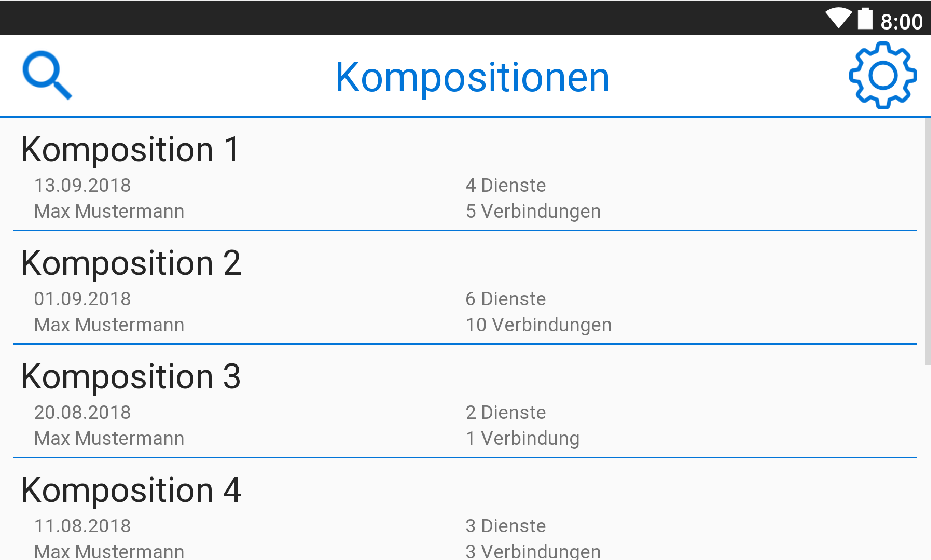
\includegraphics[width=.5\textwidth]{img/mockup_list}}
		%\caption{Listenansicht in der Android-App}
		\label{fig:mock-list}

		&In der Listenansicht werden dem Nutzer alle für ihn sichtbaren Kompositionen mit einigen Informationen (Ersteller, Erstellungsdatum, ...) angezeigt. Falls er nicht eingeloggt ist, sieht er nur die öffentlichen Kompositionen. Durch ein Tippen auf das Lupen-Symbol besteht die Möglichkeit, die Liste zu filtern. Durch das Antippen des Zahnrad-Symbols gelangt der Nutzer in ein Menü, in dem er sich unter anderem ein- und ausloggen kann.

		\\ \hline \\
		\raisebox{-.9\height}[0pt][0pt]{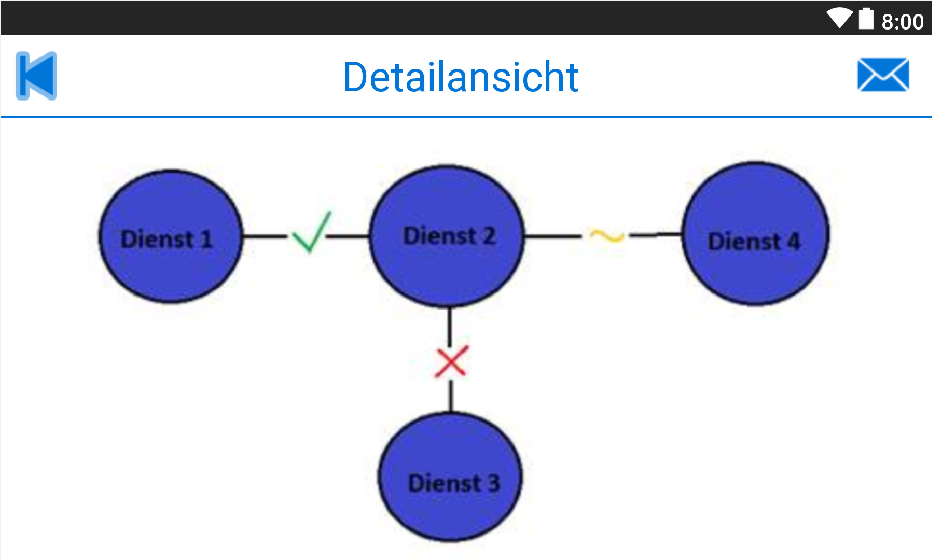
\includegraphics[width=.5\textwidth]{img/mockup_detail}}
		%\caption{Detailansicht in der Android-App}
		\label{fig:mock-detail}

		&
		Durch das Antippen einer Komposition aus der Listenansicht wird die Detailansicht geöffnet. Hier wird die Komposition als Graph dargestellt. (Fehlende) Kompatibilität wird an den Verbindungen gekennzeichnet. Mit dem Brief-Symbol kann die angezeigte Komposition verschickt werden.  Dabei wird ein PDF erstellt, das sowohl den Graphen als auch einige Details in textueller Form enthält.

	\end{tabularx}

	\caption{Mockup der Android-App}
	\label{fig:app-mockup}
\end{figure}


\begin{figure}[h]
	\centering
	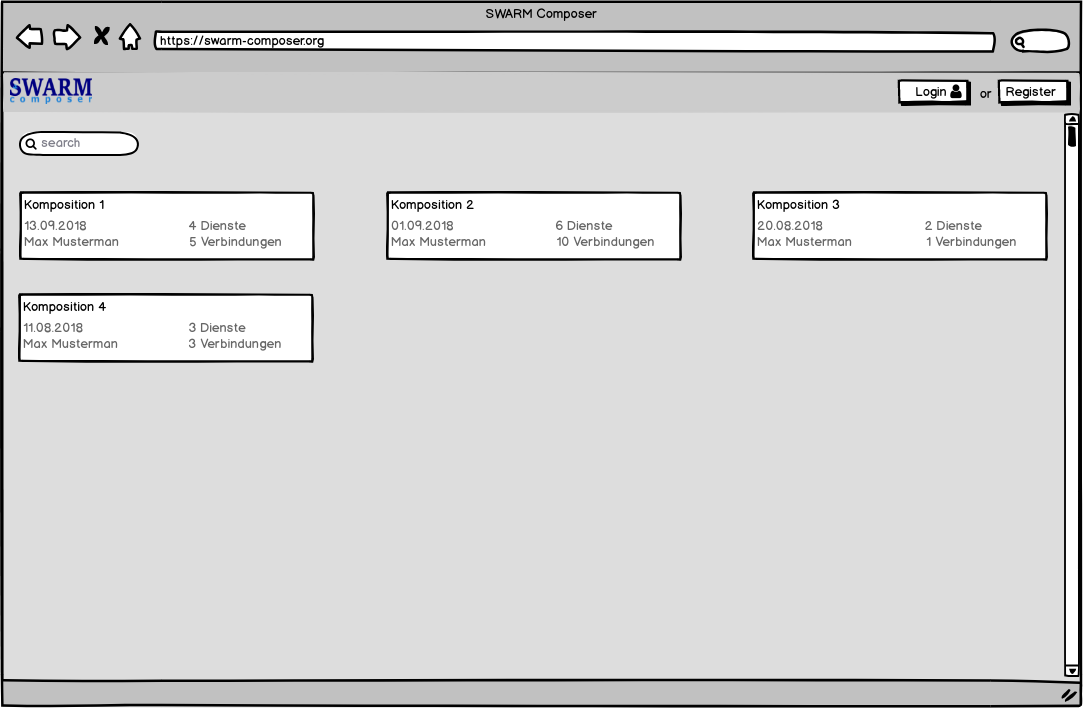
\includegraphics[width=\textwidth]{img/kompositionen}
	\caption{
            Dies ist die konzipierte Startseite. Nicht eingeloggte Nutzende bekommen alle
            öffentlich einsehbaren Kompositionen angezeigt. Durch das Drücken
            auf eine Komposition wird der Nutzende zur Bearbeitungsseite weitergeleitet.
        }
	\label{fig:kompositionen}
\end{figure}

\begin{figure}[h]
	\centering
	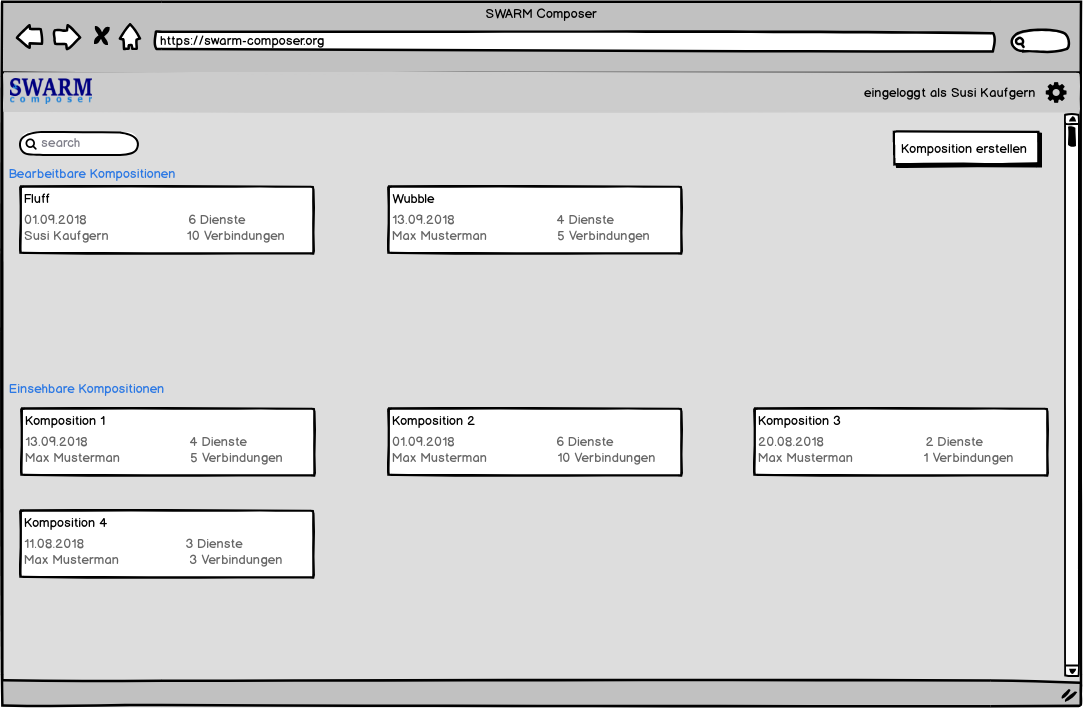
\includegraphics[width=\textwidth]{img/kompositionen_eingeloggt}
	\caption{
          Eingeloggte Nutzende können zusätzlich zu den ihnen sichtbaren Kompositionen
          auch noch für sie bearbeitbare Kompositionen getrennt sehen.
        }
	\label{fig:kompositionen-eingeloggt}
\end{figure}

\begin{figure}[h]
	\centering
	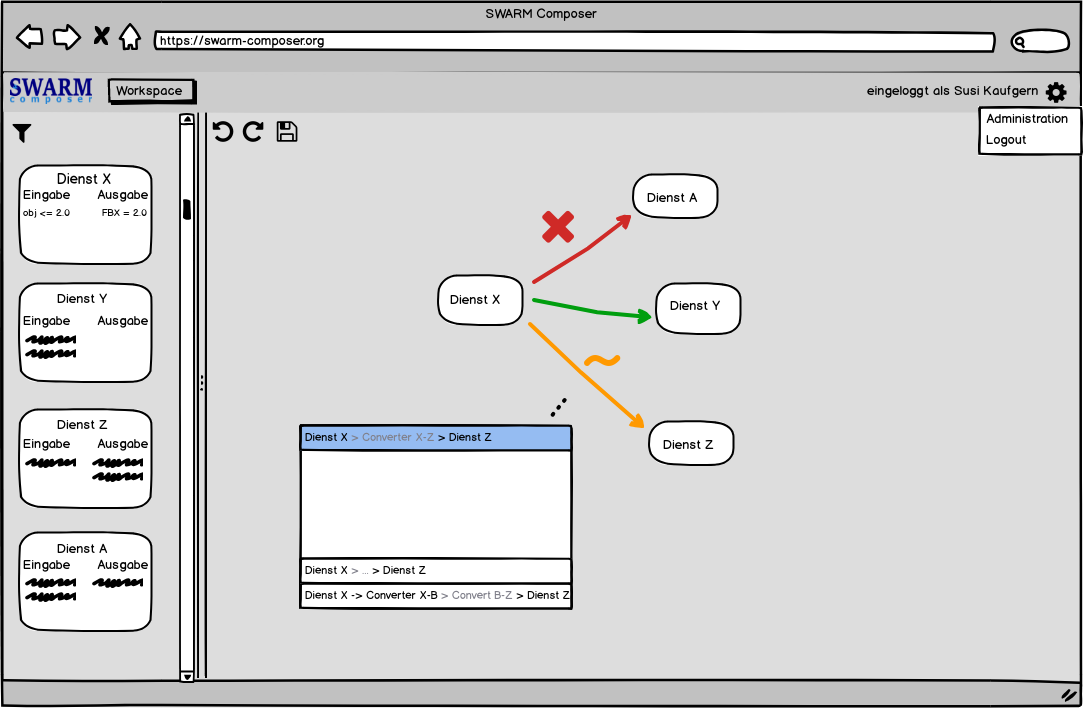
\includegraphics[width=\textwidth]{img/editor}
	\caption{
            Hier können eingeloggte Nutzer eine zuvor gewählte Komposition
            bearbeiten. Dies beinhaltet das Einfügen und Löschen von Diensten durch
            Drag-and-Drop. Weiterhin werden sowohl inkompatible Verbindungen
            als auch Alternativvorschläge grafisch hervorgehoben.
        }
	\label{fig:editor-web}
\end{figure}

\begin{figure}[h]
	\centering
	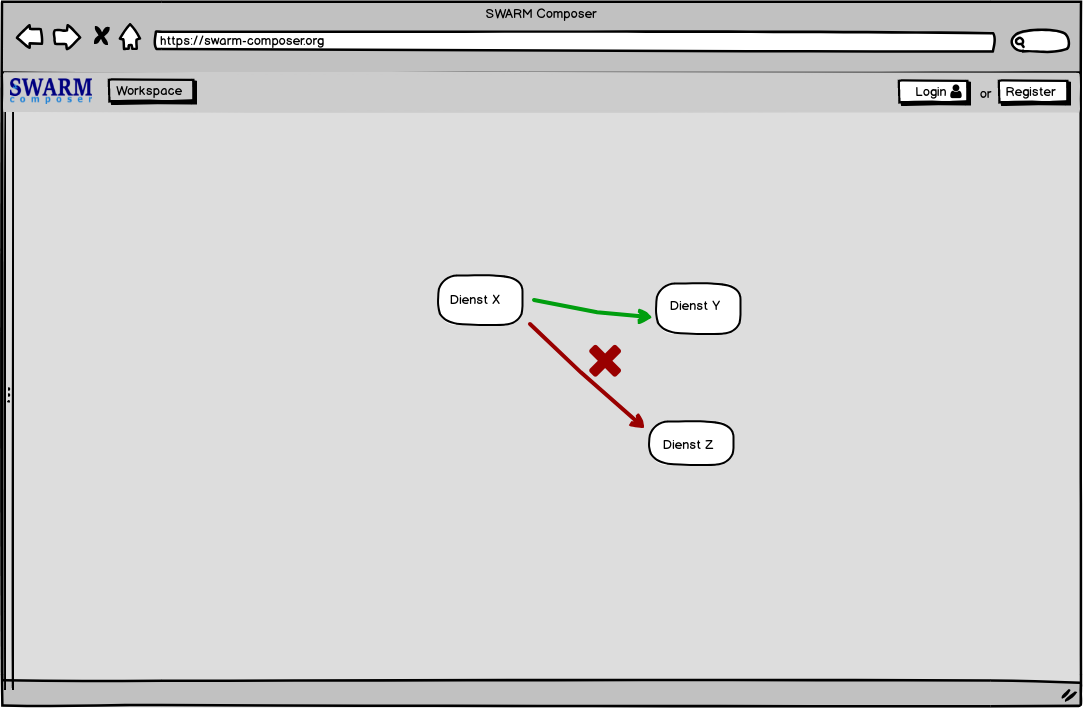
\includegraphics[width=\textwidth]{img/nichtangemeldet}
	\caption{
          Nicht angemeldete Nutzende können Kompositionen anschauen, jedoch nicht bearbeiten
        }
	\label{fig:nichtangemeldet}
\end{figure}

\begin{figure}[h]
	\centering
	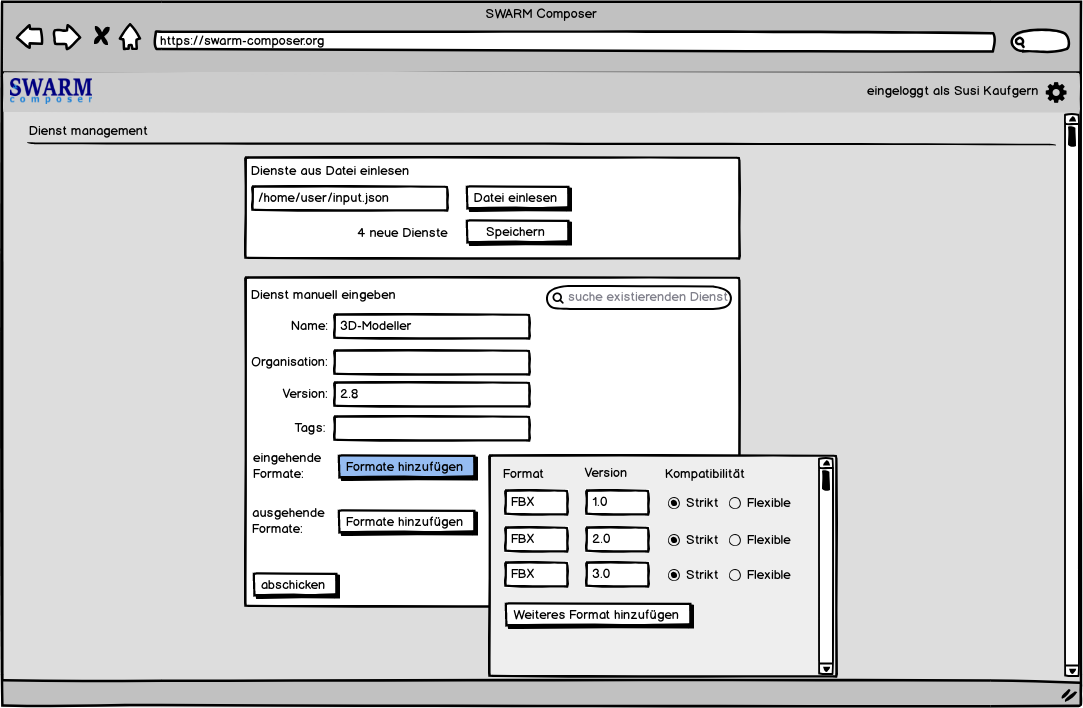
\includegraphics[width=\textwidth]{img/admin}
	\caption{
            Hier kann einE AdministratorIn neue Dienste in das System einpflegen.
            Er/Sie hat die Wahl mehrere Dienste aus einer JSON Datei einzulesen
            oder einen neuen manuell einzupflegen. Mit dem Suchfeld kann nach Diensten
            im System gesucht werden und über die gleiche Maske verändert werden.
        }
	\label{fig:admin}
\end{figure}
	
	\chapter{Qualitätsanforderung}\label{chp:qualitaetsanforderung}
	\begin{table}[h]
	\centering
	\begin{tabularx}{\textwidth}{l c c c c}
		\rowcolor[HTML]{C0C0C0} 
		& \textbf{sehr wichtig} & \textbf{wichtig} & \textbf{weniger wichtig} & \textbf{unwichtig} \\
		Robustheit &  &  & x &  \\
		\rowcolor[HTML]{E7E7E7} 
		Zuverlässigkeit & x &  &  &  \\
		Wartbarkeit &  & x &  &  \\
		\rowcolor[HTML]{E7E7E7} 
		Erweiterbarkeit &  & x &  &  \\
		Benutzerfreundlichkeit & x &  &  &  \\
		\rowcolor[HTML]{E7E7E7} 
		Effizienz &  &  & x &  \\
		Anpassbarkeit &  &  & x &  \\
		\rowcolor[HTML]{E7E7E7} 
		Kompatibilität &  &  & x &  \\
		Sicherheit &  & x &  & 
	\end{tabularx}
	\caption{Qualitätsanforderungen}
	\label{tabelle:qualitaetsanforderungen}
\end{table}
	
	\chapter{Glossar}\label{chp:glossar}
	\begin{tcolorbox}
	In diesem Glossar können Akronyme und abkürzende Schreibweisen aufgelistet werden. 
	Alle verwendeten Abkürzungen innerhalb des Projekts müssen hier erläutert werden.
\end{tcolorbox}

\begin{table}[h]
	\centering
	\begin{tabularx}{\textwidth}{X X}
		\rowcolor[HTML]{C0C0C0} 
		\textbf{Abkürzung} & \textbf{Beschreibung} \\
		Abk. A & Beschreibung A \\
		\rowcolor[HTML]{E7E7E7} 
		Abk. B & Beschreibung B \\
		Abk. C & Beschreibung C \\
		\rowcolor[HTML]{E7E7E7} 
		Abk. D & Beschreibung D \\
		Abk. E & Beschreibung E \\
		\rowcolor[HTML]{E7E7E7} 
		Abk. F & Beschreibung F \\
		Abk. G & Beschreibung G
	\end{tabularx}
	\caption{Glossar}
	\label{table:glossar}
\end{table}
	
	\bibliography{references}
	\pagenumbering{gobble} % Nummerierung deaktivieren
	
\end{document}